\documentclass{assignment}

\coursetitle{Design and Analysis of Algorithms 1}
\courselabel{CPSC 413}
\exercisesheet{Home Work \#3}{}
\student{Julie Katayama - 10092143\\
Etienne Pitout - 10075802\\
Tom Crowfoot - 10037477\\
Thomas King - 10074105}
\semester{Winter 2014}
\usepackage{amsmath}
\usepackage[linesnumbered]{algorithm2e}
\usepackage{tikz}
\usetikzlibrary{arrows}

\begin{document}

\begin{center}
\renewcommand{\arraystretch}{2}
\begin{tabular}{|c|c|c|} \hline
Problem & Marks \\ \hline \hline
1 & \\ \hline
2 & \\ \hline
3 & \\ \hline \hline
Total & \\ \hline
\end{tabular}
\end{center}

\bigskip

\begin{problemlist}
\clearpage
\pbitem
\begin{problem}
Review of undirected graphs, breadth-first search, and depth-first search.\\
(a) Let $G$ be a graph whose vertices are the integers $1$ through $8$, and let the adjacency list of each vertex be given by the table below:\\
$vertex:adjacent vertices$\\
$1~~~~~:2,3,4$\\
$2~~~~~:1,3,4$\\
$3~~~~~:1,2,4$\\
$4~~~~~:1,2,3,6$\\
$5~~~~~:6,7,8$\\
$6~~~~~:4,5,7$\\
$7~~~~~:5,6,8$\\
$8~~~~~:5,7$\\
Assume that, in a traversal of $G$, the adjacent vertices of a given vertex are returned in the same order as they are listed in the above table.\\
i. Give the sequence of vertices of $G$ visited using a DFS traversal starting at vertex $1$.\\
ii. Give the sequence of vertices visited using a BFS traversal starting at vertex $1$.\\
iii. Is $G$ connected? If yes, give a shortest list of edges to remove such that the graph is no longer connected. If no, give a shortest list of edges to add such that the graph is connected.\\
iv. Does $G$ contain a cycle? Explain your answer.\\
v. Is $G$ a tree? Explain your answer.\\
(b) An undirected graph is complete if it contains an edge between every pair of distinct vertices.\\
i. What does a depth-first search tree of a complete graph look like?\\
ii. What does a breadth-first search tree of a complete graph look like?\\
(c) Let $G$ be an undirected graph with $n$ vertices named $\{0,1,...,n-1\}$ where edges are represented as an adjacency list. Describe a data structure to store the adjacency list such that we can check in $O(logn)$ time if two vertices are adjacent. Justify your answer.\\
(d) Prove or disprove. Let $G$ be a graph on $n$ nodes, where $n$ is an even number. If every node of $G$ has degree atleast $n/2$, then $G$ is connected.\\
\end{problem}
\begin{answer}
\\
For (a):\\
For i.\\
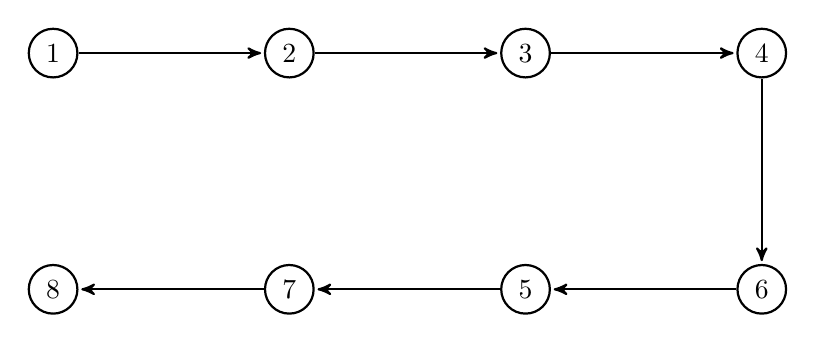
\begin{tikzpicture}[->,>=stealth',shorten >=1pt,auto,node distance=3cm,thick,node/.style={circle,draw,}]
  \node[node] (1) {1};
  \node[node] (2) [right of=1] {2};
  \node[node] (3) [right of=2] {3};
  \node[node] (4) [right of=3] {4};
  \node[node] (5) [below of=3] {5};
  \node[node] (6) [below of=4] {6};
  \node[node] (7) [below of=2] {7};
  \node[node] (8) [below of=1] {8};
  \path[node/.style]
  (1) edge node [right] {} (2)
  (2) edge node [right] {} (3)
  (3) edge node [right] {} (4)
  (4) edge node [right] {} (6)
  (5) edge node [right] {} (7)
  (6) edge node [right] {} (5)
  (7) edge node [right] {} (8);
\end{tikzpicture}
\clearpage
For ii.:\\
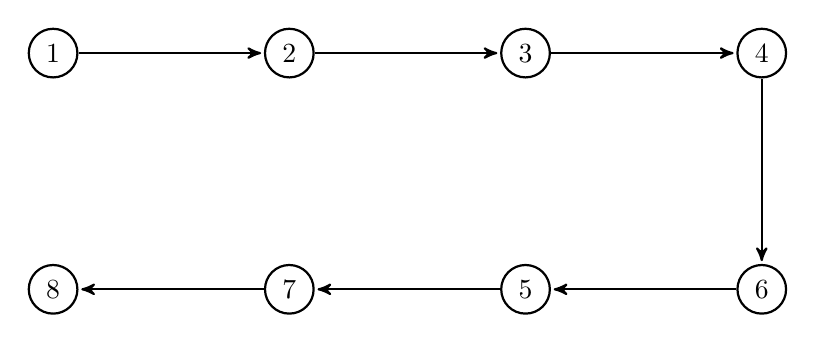
\begin{tikzpicture}[->,>=stealth',shorten >=1pt,auto,node distance=3cm,thick,node/.style={circle,draw,}]
  \node[node] (1) {1};
  \node[node] (2) [right of=1] {2};
  \node[node] (3) [right of=2] {3};
  \node[node] (4) [right of=3] {4};
  \node[node] (5) [below of=3] {5};
  \node[node] (6) [below of=4] {6};
  \node[node] (7) [below of=2] {7};
  \node[node] (8) [below of=1] {8};
  \path[node/.style]
  (1) edge node [right] {} (2)
  (2) edge node [right] {} (3)
  (3) edge node [right] {} (4)
  (4) edge node [right] {} (6)
  (5) edge node [right] {} (7)
  (6) edge node [right] {} (5)
  (7) edge node [right] {} (8);
\end{tikzpicture}
\\
For iii.\\
Yes, it is connected. If the edge between $(4,6)$ is removed, it will become unconnected.\\
For iv.\\
Yes, it contains many cycles. For example $1\rightarrow 2\rightarrow 3\rightarrow 1$\\
For v.\\
No, it is not a tree. This is because G contains at least one cycle.\\
\\
For (b):\\
For i.\\
A DFS tree of a completed graph has the appearance of a linked-list, however the order is arbitrary.\\
For ii.\\
A BFS tree of a completed graph has a node as the root and a connection to every other node in the graph. Every node which is not the root is a leaf, and the tree has a depth of 1.\\
\\For (c):\\
Create an array to hold a reference to each node in the graph. Each node will have a one-dimensional array to represent the adjacency list. Each node can then be accessed in constant time, and binary search can be used on the adjacency array to determine adjacency in $logn$ time.\\
\\
For (d):\\
True.\\
Assume that there is a graph $G$ with $n$ nodes, where every node has $deg(n/2)$.\\
For proof by contradiction, assume that $G$ is not connected.\\
Then for $v\in G$, $v$ must be connected to at least $n/2$ other nodes, so we then have a connected component of $1 + n/2$. By assumption, there is a node $x$ not connected to $v$. We also then know that $x$ must be connected to $n/2$ other nodes, and so must be in the same connected component as $v$. This then contradicts the assumption, and $G$ is connected.\\
\end{answer}
\clearpage
\pbitem
\begin{problem}
Give an algorithm to detect whether a given undirected graph contains a cycle. If the graph contains a cycle, then your algorithm should output one. The running time of your algorithm should be $O(m+n)$ for a graph with $n$ nodes and $m$ edges.\\
Give a precise statement of the problem, prove that your algorithm is correct and that the running time is $O(m+n)$.\\
\end{problem}
\begin{answer}
\\
Precondition: An undirected graph $G$, with arbitrary starting node $s$.\\
Postcondition: Either confirmation that the graph does not contain a cycle, or a cycle that was found in the graph.\\
\begin{algorithm}
  FindCycle(s):{\\
    Set Discovered[s] = true and Discovered[v] = false for all other v\;
    Initialize L[0] to consist of the single element s\;
    Set the layer counter i=0\;
    Set the current BFS tree T=\null\;
    \While{L[i] is not empty}{
      Initialize an empty list L[i+1]\;
      \For{$each~ node~ u~ in~ L[i]$}{
        Consider each edge (u,v) incident to u\;
        \If{Discovered[v] = false}{
          Set Discovered[v] = true\;
          Add edge (u,v) to the tree T\;
          Add v to the list L[i+1]\;
        }
        \If{Discovered[v] = true}{
          Add edge (u,v) to the tree T\;
          Return tree T\;
        }
      }
      Increment the layer counter i by one\;
    }
    Return that there was no cycle found\;
  }
\end{algorithm}
\\Proof: This is the BFS algorithm from the textbook, with slight modification. The algorithm from the textbook will explore an entire connected graph before terminating, and runs in $O(m+n)$ time. The only modification to the algorithm is the second if statement inside the for loop. It will not change the runtime, as the statement will execute in constant time. If the new conditional statement is always false during iterations of the algorithm, then it will have no effect. This also indicates that there were no cycles found in the graph, as during exploration the algorithm never found a previously explored node. If the new conditional statement is true at least once in the iteration of the algorithm, it will terminate, and return the first cycle that was found. A cycle is found when a previously visited node, other than the last one, is discovered during exploration.\\ 
\end{answer}
\pbitem
\begin{problem}
DAG's and topological ordering.\\
(a) Consider the directed acyclic graph G. How many topological orderings does it have?\\
$G=\{a\rightarrow b,d$\\
$~~~~b\rightarrow c$\\
$~~~~c\rightarrow f$\\
$~~~~d\rightarrow e$\\
$~~~~e\rightarrow f$\\
$~~~~f\rightarrow$\\
(b) From the text p102-104, give an algorithm in psudocode, using the data structures described, to get the $O(m+n)$ running time. Prove the algorithm does indeed have running time $O(m+n)$.\\
(c) Suppose you are given a graph that may or may not be a DAG. Extend the algorithm from 3.6 so that, given an input directed graph $G$, it outputs either a) a topological ordering, and thus $G$ is a DAG, or b) a cycle in $G$, and thus $G$ is not a DAG. The running time of your algorithm should be O(m+n) for a graph with $n$ nodes and $m$ edges.\\
Give a precise statement of the problem, prove the algorithm is correct, and the running time is $O(m+n)$.\\
\end{problem}
\begin{answer}
\\
For (a):\\
It has 6 topological orderings.\\
1: $a,b,c,d,e,f$\\
2: $a,b,d,c,e,f$\\
3: $a,b,d,e,c,f$\\
4: $a,d,e,b,c,f$\\
5: $a,d,b,e,c,f$\\
6: $a,d,b,c,e,f$\\
\clearpage
For (b):\\
Precondition: A DAG $G$, and $n$ which is the size of $G$.\\
Postcondition: A valid topological ordering for $G$.\\
\begin{algorithm}
  FindOrder(G, n):{\\
    outputArray[n]\;
    arrayPointer = 0\;
    stack\;
    \For{each node x in G}{
      Compute indegree(x)\;
      \If{indegree(x)== 0}{
        stack.push(x)\;
        outputArray[arrayPointer++]=x\;
      }
    }
    \While{$stack.top != NULL$}{
      v = stack.pop\;
      outputArray[arrayPointer++]=v\;
      \For{each edge between v and x in G}{
        indegree(x)-1\;
        \If{indegree(x)==0}{
          stack.push(x)\;
        }
      }
    }
    return outputArray\;
  }
\end{algorithm}
\\
Proof of runtime:\\
The cost of initializing the stack and array is constant. The cost to compute the indegree for each node in the DAG is $n$. As the graph is a DAG, the while loop will iterate $n$ times, once for each node. The cost of the inner for loop will be much smaller than $m$, as it will iterate for the number of edges for the current node. The cost of the for loop iterated $n$ times will then be $m$, as we will remove every edge in the graph. We then find the total cost of the algorithm to be $c + n + \sum_{i=1}^n(c)$. We can use the limit test to find the runtime bound of our algorithm.\\
We then find:
\begin{align*}
&c + n + \sum_{i=1}^n(c)\\
=&c + n + m\\
&\lim_{n\rightarrow \infty} \frac{c + n + m}{n + m}\\
=&\lim_{n\rightarrow \infty} \frac{c/n + 1 + m/n}{1 + m/n}\\
=& 1\\
\end{align*}
As the limit resolves to a constant, the runtime of this algorithm is $\Theta(n+m)$. This then implies that the algorithm also has a runtime of $O(n+m)$.\\
\clearpage
For (c):\\
Precondition: A directed graph $G$, size of $n$.\\
Postconditon: Either a valid topological ordering of $G$ and $G$ is a DAG, or a cycle found in $G$.\\
\begin{algorithm}
  FindOrderOrCycle(G, n):{\\
    outputArray[n]\;
    arrayPointer = 0\;
    stack\;
    \For{each node x in G}{
      Compute indegree(x)\;
      \If{indegree(x)== 0}{
        stack.push(x)\;
        outputArray[arrayPointer++]=x\;
      }
    }
    \While{$stack.top != NULL$}{
      v = stack.pop\;
      outputArray[arrayPointer++]=v\;
      \For{each edge between v and x in G}{
        indegree(x)-1\;
        \If{indegree(x)==0}{
          stack.push(x)\;
        }
      }
    }
    \eIf{arrayPointer == n}{
      return outputArray\;
    }{
      return FindCycleDirected(x)\;
    }
  }
\end{algorithm}
\clearpage
\begin{algorithm}
  FindCycleDirected(s):{\\
    Set Discovered[s] = true and Discovered[v] = false for all other v\;
    Initialize L[0] to consist of the single element s\;
    Set the layer counter i=0\;
    Set the current BFS tree T=\null\;
    \While{L[i] is not empty}{
      Initialize an empty list L[i+1]\;
      \For{$each~ node~ u~ in~ L[i]$}{
        Consider each edge (u,v) incident to u\;
        \If{Discovered[v] = false}{
          Set Discovered[v] = true\;
          Add edge (u,v) to the tree T\;
          Add v to the list L[i+1]\;
        }
        \If{Discovered[v] = true}{
          Add edge (u,v) to the tree T\;
          stack.push(v)\;
          \While{stack.top != null}{
            \For{$each~node~u~adjacent~to~stack.top$}{
              stack.push(u)\;
              Add edge (u,stack.top) to the tree T\;
              \If{u==s}{
                Return tree T\;
              }
            }
            stack.pop\;
          }
        }
      }
      Increment the layer counter i by one\;
    }
  }
\end{algorithm}
Proof of runtime:\\
This algorithm is a modification of the algorithm given in question 3(b). The only difference occurs when the algorithm is given a graph with a cycle. When this happens, this algorithm terminates and calls a slightly modified version of the algorithm in question 2. The modification to the algorithm from question two is to add a basic depth first search traversal in the case the BFS encounters a node it has already examined. When this happens, it uses the DFS to try to reach the start of the graph. If it is successful, we then know there is a path from the start to the node which we are re-examining, and a path from that node back to the start which gives us a cycle. It is proved in the book that DFS has a runtime of $O(n+m)$ in worst case, so the runtime of the algorithm after the modification will have the cost of the original algorithm plus the cost of DFS, so it will be $O(n+m+n+m)$ in worst case. The algorithm from 3(b) was proved to run in $O(n+m)$ time. In worst case, we will have to run both algorithms to completion, and thus we find:
\begin{align*}
&(n+m) + (n+m+n+m)\\
=&3n + 3m\\
&\lim_{n\rightarrow \infty} \frac{3n+3m}{n+m}\\
=&\lim_{n\rightarrow \infty} \frac{3+3m/n}{1+m/n}\\
=&3\\
\end{align*}
Thus the algorithm runs in $\Theta (n+m)$, as the limit resolves to a constant. This then implies that the algorithm is in $O(n+m)$.\\
Proof of correctness:\\
The proof of correctness for the algorithm will be the same as for questions 2 and 3b. The algorithm from 3b starts by examining a node with no incoming edges. It then removes this node from the graph and updates the number of incoming edges for the remaining nodes in the graph. It repeats this process until either the graph is empty, in which case we now have a topological order and can stop, or there are no more nodes in the graph with an incoming degree of 0, so we cannot find a topological ordering. As proved in the text, a graph has a topological ordering if and only if it is acyclic. We then know that the graph must have a cycle, as we could not find a topological ordering. The algorithm then calls the modified algorithm from question 2 on the remaining graph to find that cycle. The algorithm will build a tree using BFS until it encounters a node it has already examined. As the graph is directed, this is not enough to indicate that a cycle has been found, so it must then attempt to find a path back to the node that the BFS started on. If it is unable to do so, then finding this previously explored node was a false alarm. In this situation, the algorithm will continue exploring in BFS. If it was possible to find a path from the previously explored node to the start, then there is a cycle, and the algorithm will terminate.
\end{answer}

\end{problemlist}
\end{document}
